% Automatisch gegenereerd door scripts/generate_diagram.py — niet handmatig bewerken.
\documentclass[tikz,border=4mm]{standalone}
\usetikzlibrary{arrows.meta,positioning,calc}
\definecolor{csorbox}{HTML}{EDF2FB}
\definecolor{csorline}{HTML}{1B3A6B}
\definecolor{extbox}{HTML}{FBF2E3}
\definecolor{extline}{HTML}{8A5A00}
\begin{document}
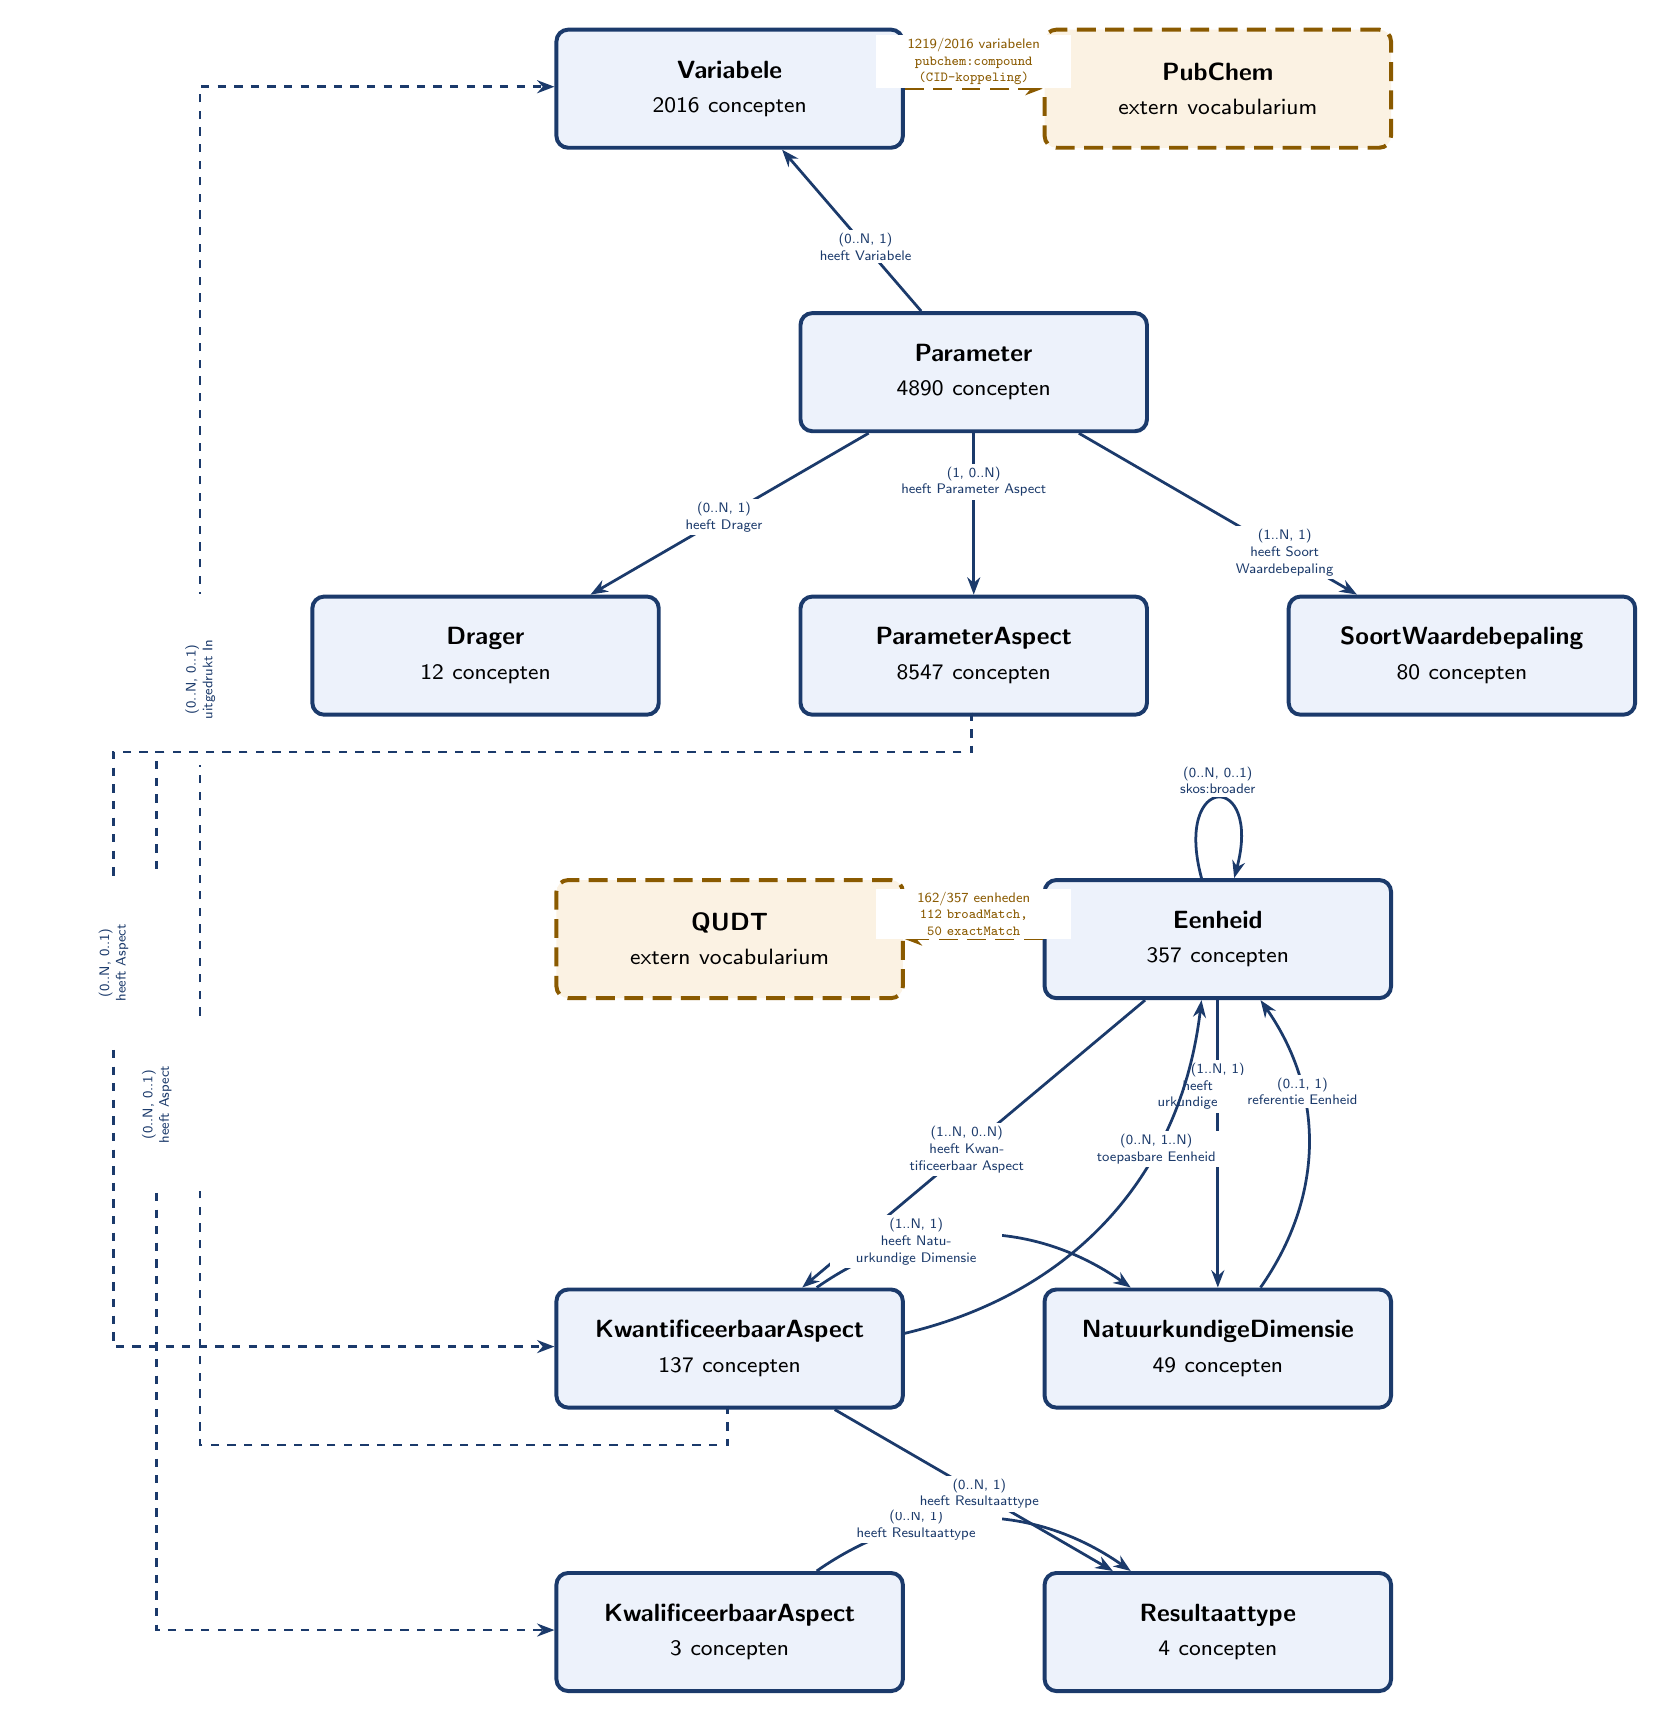
\begin{tikzpicture}[
  every node/.style={font=\sffamily\small},
  klasse/.style={draw=csorline, fill=csorbox, line width=0.5mm, rounded corners=1.5mm,
    minimum width=4.4cm, minimum height=1.5cm, text width=3.9000000000000004cm,
    align=center, anchor=north west},
  extern/.style={draw=extline, fill=extbox, line width=0.5mm, rounded corners=1.5mm,
    dash pattern=on 2.4mm off 1.2mm,
    minimum width=4.4cm, minimum height=1.5cm, text width=3.9000000000000004cm,
    align=center, anchor=north west},
  rel/.style={-{Stealth[length=2.2mm]}, line width=0.35mm, csorline},
  extrel/.style={-{Stealth[length=2.2mm]}, line width=0.35mm, extline,
    dash pattern=on 2.4mm off 1.2mm},
  lbl/.style={font=\sffamily\tiny, fill=white, inner sep=0.4mm, align=center,
    text=csorline, text width=2.1cm},
  extlbl/.style={font=\sffamily\tiny, fill=white, inner sep=0.4mm, align=center,
    text=extline, text width=2.4cm}
]
\node[klasse] (Drager) at (0.000,-7.200) {\textbf{Drager}\\[0.5mm]\footnotesize 12 concepten};
\node[klasse] (Eenheid) at (9.300,-10.800) {\textbf{Eenheid}\\[0.5mm]\footnotesize 357 concepten};
\node[klasse] (KwalificeerbaarAspect) at (3.100,-19.600) {\textbf{KwalificeerbaarAspect}\\[0.5mm]\footnotesize 3 concepten};
\node[klasse] (KwantificeerbaarAspect) at (3.100,-16.000) {\textbf{KwantificeerbaarAspect}\\[0.5mm]\footnotesize 137 concepten};
\node[klasse] (NatuurkundigeDimensie) at (9.300,-16.000) {\textbf{NatuurkundigeDimensie}\\[0.5mm]\footnotesize 49 concepten};
\node[klasse] (Parameter) at (6.200,-3.600) {\textbf{Parameter}\\[0.5mm]\footnotesize 4890 concepten};
\node[klasse] (ParameterAspect) at (6.200,-7.200) {\textbf{ParameterAspect}\\[0.5mm]\footnotesize 8547 concepten};
\node[extern] (PubChem) at (9.300,-0.000) {\textbf{PubChem}\\[0.5mm]\footnotesize extern vocabularium};
\node[extern] (QUDT) at (3.100,-10.800) {\textbf{QUDT}\\[0.5mm]\footnotesize extern vocabularium};
\node[klasse] (Resultaattype) at (9.300,-19.600) {\textbf{Resultaattype}\\[0.5mm]\footnotesize 4 concepten};
\node[klasse] (SoortWaardebepaling) at (12.400,-7.200) {\textbf{SoortWaardebepaling}\\[0.5mm]\footnotesize 80 concepten};
\node[klasse] (Variabele) at (3.100,-0.000) {\textbf{Variabele}\\[0.5mm]\footnotesize 2016 concepten};
\draw[rel] (Eenheid) -- node[lbl, pos=0.52] {(1..N, 0..N)\\heeft Kwantificeerbaar Aspect} (KwantificeerbaarAspect);
\draw[rel] (Eenheid) -- node[lbl, pos=0.3] {(1..N, 1)\\heeft Natuurkundige Dimensie} (NatuurkundigeDimensie);
\draw[rel] (Eenheid) edge[loop above, looseness=6, min distance=14mm] node[lbl, pos=0.5] {(0..N, 0..1)\\skos:broader} (Eenheid);
\draw[rel] (KwalificeerbaarAspect) to[bend left=35] node[lbl, pos=0.32] {(0..N, 1)\\heeft Resultaattype} (Resultaattype);
\draw[rel] (KwantificeerbaarAspect) to[bend left=35] node[lbl, pos=0.32] {(1..N, 1)\\heeft Natuurkundige Dimensie} (NatuurkundigeDimensie);
\draw[rel] (KwantificeerbaarAspect) -- node[lbl, pos=0.52] {(0..N, 1)\\heeft Resultaattype} (Resultaattype);
\draw[rel] (KwantificeerbaarAspect) to[bend right=35] node[lbl, pos=0.68] {(0..N, 1..N)\\toepasbare Eenheid} (Eenheid);
\draw[rel, dashed] (5.300,-17.500) -- (5.300,-18.000) -- (-1.400,-18.000) -- (-1.400,-0.750) -- (3.100,-0.750);
\node[lbl, anchor=south] at (-1.400,-9.375) {\rotatebox{90}{\begin{minipage}{2.1cm}\centering (0..N, 0..1)\\uitgedrukt In\end{minipage}}};
\draw[rel] (NatuurkundigeDimensie) to[bend right=35] node[lbl, pos=0.68] {(0..1, 1)\\referentie Eenheid} (Eenheid);
\draw[rel] (Parameter) -- node[lbl, pos=0.52] {(0..N, 1)\\heeft Drager} (Drager);
\draw[rel] (Parameter) -- node[lbl, pos=0.3] {(1, 0..N)\\heeft Parameter Aspect} (ParameterAspect);
\draw[rel] (Parameter) -- node[lbl, pos=0.74] {(1..N, 1)\\heeft Soort Waardebepaling} (SoortWaardebepaling);
\draw[rel] (Parameter) -- node[lbl, pos=0.4] {(0..N, 1)\\heeft Variabele} (Variabele);
\draw[rel, dashed] (8.400,-8.700) -- (8.400,-9.200) -- (-1.950,-9.200) -- (-1.950,-20.350) -- (3.100,-20.350);
\node[lbl, anchor=south] at (-1.950,-14.775) {\rotatebox{90}{\begin{minipage}{2.1cm}\centering (0..N, 0..1)\\heeft Aspect\end{minipage}}};
\draw[rel, dashed] (8.400,-8.700) -- (8.400,-9.200) -- (-2.500,-9.200) -- (-2.500,-16.750) -- (3.100,-16.750);
\node[lbl, anchor=south] at (-2.500,-12.975) {\rotatebox{90}{\begin{minipage}{2.1cm}\centering (0..N, 0..1)\\heeft Aspect\end{minipage}}};
\draw[extrel] (Eenheid) -- (QUDT);
\node[extlbl, above] at ($(Eenheid)!0.5!(QUDT)$) {162/357 eenheden\\{\ttfamily 112 broadMatch, 50 exactMatch}};
\draw[extrel] (Variabele) -- (PubChem);
\node[extlbl, above] at ($(Variabele)!0.5!(PubChem)$) {1219/2016 variabelen\\{\ttfamily pubchem:compound (CID-koppeling)}};
\end{tikzpicture}
\end{document}
